\chapter{Wielowymiarowy regulator PID}
\label{pro_pid}

W ramach kolejnego zadania zaimplementowaliśmy wielowymiarowy regulator 
PID o 4 wejściach i 3 wyjściach. 

\section{Implementacja wielowymiarowego regulatora PID}
\label{pro_pid_implementacja}

Implementacja regulatora wielowymiarowego
jest podobna do zwykłego regulatora jednowymiarowego, z tą różnicą
że każdy parametr skalarny $K_{\mathrm{p}}$, $T_{\mathrm{i}}$ i $T_{\mathrm{d}}$
jest teraz wektorem o takiej ilości elementów jaka jest liczba wejść. \\

\begin{lstlisting}[style=custommatlab,frame=single,label={pro_pid_parametry},caption={Przykładowa definicja parametrów regulatora},captionpos=b]
%% Parametry regulatorow ciaglych
K = [1 0 1 1];
Ti = [3 99999 99999 100];
Td = [0.05 0 0 0];

%% Parametry regulatorow dyskretnych
r0 = zeros(N,1);
r1 = zeros(N,1);
r2 = zeros(N,1);

for i=1:N
    r0(i) = K(i)*(1 + T/(2*Ti(i)) + Td(i)/T);
    r1(i) = K(i)*(T/(2*Ti(i)) - (2*Td(i))/T - 1);
    r2(i) = (K(i)*Td(i))/T;
end
\end{lstlisting}

W przypadku obiektów wielowymiarowych, należy dokonać decyzji, które uchyby 
powinny oddziaływać na które wejście. W przypadku naszej implementacji zdecydowaliśmy 
się na wprowadzenie macierzy połączeń, która opisuje związek wejścia z wyjściem. \\

\begin{lstlisting}[style=custommatlab,frame=single,label={pro_pid_conn_matrix},caption={Przykładowa macierz połączeń},captionpos=b]
% macierz polaczen, okresla z jaka waga jest brany dany uchyb do regulatora
CONNECTION_MATRIX = [1 0 0;
                     0 0 0;
                     0 1 0;
                     0 0 1];
\end{lstlisting}

W przypadku macierzy opisanej w \ref{pro_pid_conn_matrix}, uchyb wyjścia pierwszego
wchodzi wchodzi na wejście regulatora pierwszego, uchyba wyjścia drugiego wchodzi
na wejście regulatora trzeciego a uchyb wyjścia trzeciego wchodzi na wejście regulatora 
czwartego. Wejście drugie w tym przypadku pozostaje niesterowane.\\

Tak opisana struktura regulatora wielowymiarowego pozwala nie tylko na binarne opisanie struktury ale 
umożliwia również wpisywanie niezerowych wag, np. uchyb pierwszy wchodzi na wejście regulatora pierwszego
z wagą $\num{0.8}$ a na wejście regulatora drugiego z wagą $\num{0.2}$. Pozwala to 
na projektowanie bardziej wyrafinowanych algorytmów regulacji.

\begin{figure}[p!]
    \centering
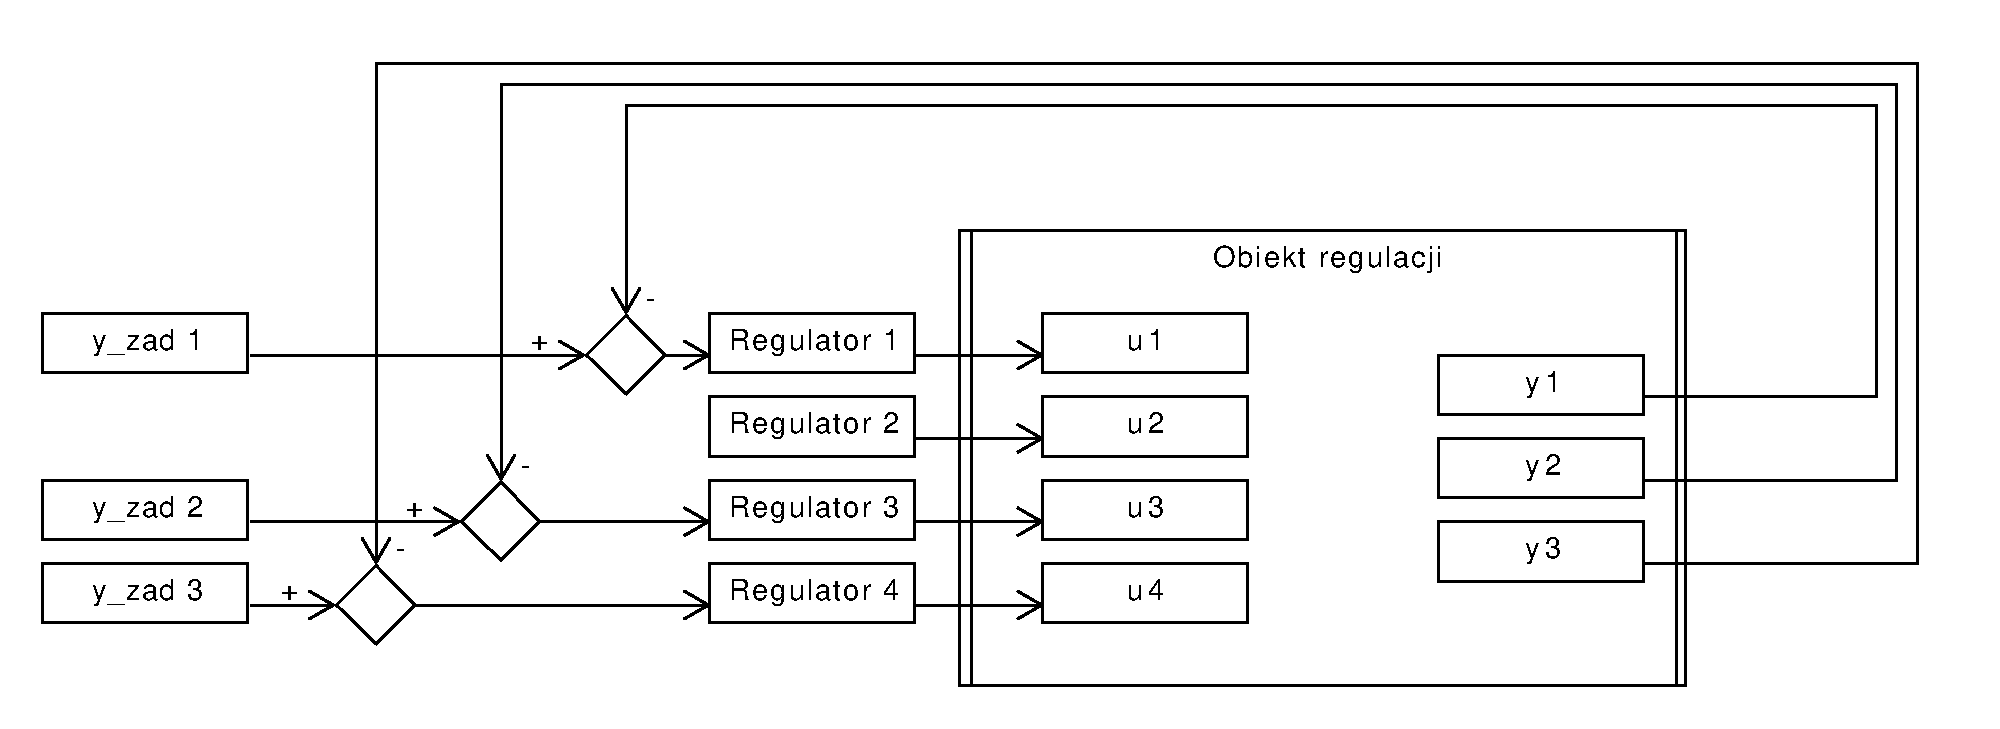
\includegraphics[scale=0.7, angle=90]{uklad_regulacji_pid.pdf}
\caption{Struktura regulacji opisywana przez macierz z listingu \ref{pro_pid_conn_matrix}}
\end{figure}

\FloatBarrier

Mając gotową opisaną strukturę regulatora wielowymiarowego oraz dobrane parametry,
możliwa jest implementacja pętli obliczającej nowe sterowania. \\

\begin{lstlisting}[style=custommatlab,frame=single,label={pro_pid_petla},caption={Pętla obliczająca sterowania wielowymiarowego regulatora PID},captionpos=b]
%% Petla symulujaca dzialanie cyfrowego algorytmu PID w wersji MIMO
for k = 5:SIM_LEN  
  [y1, y2, y3] = symulacja_obiektu1(inputs(k-1, 1), inputs(k-2, 1), ...
                                    inputs(k-3, 1), inputs(k-4, 1), ...
                                    inputs(k-1, 2), inputs(k-2, 2), ...
                                    inputs(k-3, 2), inputs(k-4, 2), ...
                                    inputs(k-1, 3), inputs(k-2, 3), ...
                                    inputs(k-3, 3), inputs(k-4, 3), ...
                                    inputs(k-1, 4), inputs(k-2, 4), ...
                                    inputs(k-3, 4), inputs(k-4, 4), ...
                                    outputs(k-1, 1), outputs(k-2, 1), ...
                                    outputs(k-3, 1), outputs(k-4, 1), ...
                                    outputs(k-1, 2), outputs(k-2, 2), ...
                                    outputs(k-3, 2), outputs(k-4, 2), ...
                                    outputs(k-1, 3), outputs(k-2, 3), ...
                                    outputs(k-3, 3), outputs(k-4, 3));
  outputs(k, :) = [y1 y2 y3];                        
  errors(k, :) = setpoints(k, :) - outputs(k, :); % obliczenie uchybow    

  % obliczenie nowych sterowan
  for i=1:N
    error = CONNECTION_MATRIX(i,:)*(errors(k-2:k, :)');
    inputs(k,i) = r2(i)*error(1) + r1(i)*error(2) + ...
                  r0(i)*error(3) + inputs(k-1, i); 
  end
end
\end{lstlisting}

\section{Strojenie wielowymiarowego regulatora PID z binarną macierzą połączeń}
\label{pro_pid_bin_conn}

Strojenie wielowymiarowego regulatora PID nie należy do spraw prostych.
W dalszej części tej sekcji opisaliśmy proces eksperymentalnego 
doboru parametrów regulatora.

\subsection{Konfiguracja z najmocniejszymi wzmocnieniami}
\label{pro_pid_konf1}

Analizując odpowiedzi na poszczególne skoki sygnałów wejściowych, zdecydowaliśmy się
sprawdzić konfigurację wejść i wyjść w której:\\

\begin{itemize}
    \item uchyb wyjścia pierwszego wchodzi na wejście pierwsze
    \item uchyb wyjścia drugiego wchodzi na wejście trzecie
    \item uchyb wyjścia trzeciego wchodzi na wejście czwarte
    \item wejście drugie pozostaje niesterowane
\end{itemize}

\noindent Macierz połączeń w tym przypadku miała postać: \\

\[
C =
\begin{bmatrix}
    1 & 0 & 0 \\
    0 & 0 & 0 \\
    0 & 1 & 0 \\
    0 & 0 & 1 
\end{bmatrix}
\]

W pierwszej kolejności sprawdziliśmy jak układ regulacji zachowa się w 
sytuacji gdy proces będzie sterowany regulatorami typu P o wzmocnieniu 
jednostkowym.

\begin{center}
$K^{\num{1}}_{\mathrm{p}} = \num{1.0}$, $T^{\num{1}}_{\mathrm{i}} = \infty$, $T^{\num{1}}_{\mathrm{d}} = \num{0.0}$ \\
$K^{\num{2}}_{\mathrm{p}} = \num{1.0}$, $T^{\num{2}}_{\mathrm{i}} = \infty$, $T^{\num{2}}_{\mathrm{d}} = \num{0.0}$ \\
$K^{\num{3}}_{\mathrm{p}} = \num{1.0}$, $T^{\num{3}}_{\mathrm{i}} = \infty$, $T^{\num{3}}_{\mathrm{d}} = \num{0.0}$ \\
$K^{\num{4}}_{\mathrm{p}} = \num{1.0}$, $T^{\num{4}}_{\mathrm{i}} = \infty$, $T^{\num{4}}_{\mathrm{d}} = \num{0.0}$ \\
\end{center}

%% wyjscia 

\begin{figure}
    \centering
    \begin{subfigure}[b]{\textwidth}
        \centering
        \resizebox{\linewidth}{!}{
            \begin{tikzpicture}
                \begin{axis}[
                    width=0.98\textwidth,
                    height=7cm,
                    xmin=0.0,xmax=1000,ymin=-0.5,ymax=2,
                    xlabel={$k$},
                    ylabel={$y_{\mathrm{1}}[k]$},
                    legend pos=south east,
                    y tick label style={/pgf/number format/1000 sep=},
                    ] 
                    \addlegendentry{$y_{\mathrm{1}}[k]$},
                    \addlegendentry{$y_{\mathrm{1}}^{\mathrm{zad}}[k]$},
                
                    \addlegendimage{no markers,red}
                    \addlegendimage{no markers,blue}
                
                    \addplot[red, semithick] file{../data/project/zad4/pid/konf1_wzmocnienia_jednostkowe/output_1.csv};  
                    \addplot[blue, semithick] file{../data/project/zad4/pid/konf1_wzmocnienia_jednostkowe/stpt_1.csv};
                    
                    \end{axis}
            \end{tikzpicture}
        }
        \end{subfigure}

        \begin{subfigure}[b]{\textwidth}
            \centering
            \resizebox{\linewidth}{!}{
                \begin{tikzpicture}
                    \begin{axis}[
                        width=0.98\textwidth,
                        height=7cm,
                        xmin=0.0,xmax=1000,ymin=-0.5,ymax=2,
                        xlabel={$k$},
                        ylabel={$y_{\mathrm{2}}[k]$},
                        legend pos=south east,
                        y tick label style={/pgf/number format/1000 sep=},
                        ] 
                        \addlegendentry{$y_{\mathrm{2}}[k]$},
                        \addlegendentry{$y_{\mathrm{2}}^{\mathrm{zad}}[k]$},
                    
                        \addlegendimage{no markers,red}
                        \addlegendimage{no markers,blue}
                    
                        \addplot[red, semithick] file{../data/project/zad4/pid/konf1_wzmocnienia_jednostkowe/output_2.csv};  
                        \addplot[blue, semithick] file{../data/project/zad4/pid/konf1_wzmocnienia_jednostkowe/stpt_2.csv};
                        
                        \end{axis}
                \end{tikzpicture}
            }
        \end{subfigure}

        \begin{subfigure}[b]{\textwidth}
            \centering
            \resizebox{\linewidth}{!}{
                \begin{tikzpicture}
                    \begin{axis}[
                        width=0.98\textwidth,
                        height=7cm,
                        xmin=0.0,xmax=1000,ymin=-0.5,ymax=2,
                        xlabel={$k$},
                        ylabel={$y_{\mathrm{3}}[k]$},
                        legend pos=south east,
                        y tick label style={/pgf/number format/1000 sep=},
                        ] 
                        \addlegendentry{$y_{\mathrm{3}}[k]$},
                        \addlegendentry{$y_{\mathrm{3}}^{\mathrm{zad}}[k]$},
                    
                        \addlegendimage{no markers,red}
                        \addlegendimage{no markers,blue}
                    
                        \addplot[red, semithick] file{../data/project/zad4/pid/konf1_wzmocnienia_jednostkowe/output_3.csv};  
                        \addplot[blue, semithick] file{../data/project/zad4/pid/konf1_wzmocnienia_jednostkowe/stpt_3.csv};
                        
                        \end{axis}
                \end{tikzpicture}
            }
        \end{subfigure}
        \caption{Wyjścia procesu wielowymiarowego}
        \label{pro_pid_2_out}
\end{figure}

%% wejscia 

\begin{figure}
    \centering
    \begin{subfigure}[b]{\textwidth}
        \centering
        \resizebox{\linewidth}{!}{
            \begin{tikzpicture}
                \begin{axis}[
                    width=0.98\textwidth,
                    height=6cm,
                    xmin=0.0,xmax=1000,ymin=-3,ymax=3,
                    xlabel={$k$},
                    ylabel={$u_{\mathrm{1}}[k]$},
                    legend pos=south east,
                    y tick label style={/pgf/number format/1000 sep=},
                    ] 
                    \addlegendentry{$u_{\mathrm{1}}[k]$},
                    \addlegendimage{no markers,blue}
                    \addplot[const plot, blue, semithick] file{../data/project/zad4/pid/konf1_wzmocnienia_jednostkowe/input_1.csv};  
                \end{axis}
            \end{tikzpicture}
        }
    \end{subfigure}

    \begin{subfigure}[b]{\textwidth}
        \centering
        \resizebox{\linewidth}{!}{
            \begin{tikzpicture}
                \begin{axis}[
                    width=0.98\textwidth,
                    height=6cm,
                    xmin=0.0,xmax=1000,ymin=-3,ymax=3,
                    xlabel={$k$},
                    ylabel={$u_{\mathrm{2}}[k]$},
                    legend pos=south east,
                    y tick label style={/pgf/number format/1000 sep=},
                    ] 
                    \addlegendentry{$u_{\mathrm{2}}[k]$},
                    \addlegendimage{no markers,blue}
                    \addplot[const plot, blue, semithick] file{../data/project/zad4/pid/konf1_wzmocnienia_jednostkowe/input_2.csv};  
                \end{axis}
            \end{tikzpicture}
        }
    \end{subfigure}

    \begin{subfigure}[b]{\textwidth}
        \centering
        \resizebox{\linewidth}{!}{
            \begin{tikzpicture}
                \begin{axis}[
                    width=0.98\textwidth,
                    height=6cm,
                    xmin=0.0,xmax=1000,ymin=-3,ymax=3,
                    xlabel={$k$},
                    ylabel={$u_{\mathrm{3}}[k]$},
                    legend pos=south east,
                    y tick label style={/pgf/number format/1000 sep=},
                    ] 
                    \addlegendentry{$u_{\mathrm{3}}[k]$},
                    \addlegendimage{no markers,blue}
                    \addplot[const plot, blue, semithick] file{../data/project/zad4/pid/konf1_wzmocnienia_jednostkowe/input_3.csv};  
                \end{axis}
            \end{tikzpicture}
        }
    \end{subfigure}

    \begin{subfigure}[b]{\textwidth}
        \centering
        \resizebox{\linewidth}{!}{
            \begin{tikzpicture}
                \begin{axis}[
                    width=0.98\textwidth,
                    height=6cm,
                    xmin=0.0,xmax=1000,ymin=-3,ymax=3,
                    xlabel={$k$},
                    ylabel={$u_{\mathrm{4}}[k]$},
                    legend pos=south east,
                    y tick label style={/pgf/number format/1000 sep=},
                    ] 
                    \addlegendentry{$u_{\mathrm{4}}[k]$},
                    \addlegendimage{no markers,blue}
                    \addplot[const plot, blue, semithick] file{../data/project/zad4/pid/konf1_wzmocnienia_jednostkowe/input_4.csv};  
                \end{axis}
            \end{tikzpicture}
        }
    \end{subfigure}

    \caption{Wejścia procesu wielowymiarowego}
    \label{pro_pid_2_in}
\end{figure}
\FloatBarrier

Algorytm regulacji z tak dobranymi parametrami średnio radzi sobie z 
regulacją badanego obiektu. Wynika to z faktu błędnego dobrania parametrów 
regulatora oraz braku sterowania jednego z wejść. Wskaźniki jakości liczone względem 
każdego z wyjść wyniosły: 

\[
\begin{bmatrix}
    E_{\mathrm{1}} \\
    E_{\mathrm{2}} \\
    E_{\mathrm{3}} 
\end{bmatrix}
= 
\begin{bmatrix}
    \num{31.462} \\
    \num{151.32} \\
    \num{89.142}
\end{bmatrix}
\]

Sumaryczny wskaźnik jakości, liczony jako suma wskaźników składowych, 
wyniósł $\bar{E} = \num{271.92}$\\

\vspace{2cm}

W kolejnej próbie zdecydowaliśmy sie na zwiększenie parametrów $K^{i}_{\mathrm{p}}$, tak aby
lepiej wspomagały wzmocnienia obsługiwanych torów sterowania. Zdecydowaliśmy się na następujący
zestaw parametrów 

\begin{center}
    $K^{\num{1}}_{\mathrm{p}} = \num{3.0}$, $T^{\num{1}}_{\mathrm{i}} = \infty$, $T^{\num{1}}_{\mathrm{d}} = \num{0.0}$ \\
    $K^{\num{2}}_{\mathrm{p}} = \num{0.0}$, $T^{\num{2}}_{\mathrm{i}} = \infty$, $T^{\num{2}}_{\mathrm{d}} = \num{0.0}$ \\
    $K^{\num{3}}_{\mathrm{p}} = \num{2.0}$, $T^{\num{3}}_{\mathrm{i}} = \infty$, $T^{\num{3}}_{\mathrm{d}} = \num{0.0}$ \\
    $K^{\num{4}}_{\mathrm{p}} = \num{4.0}$, $T^{\num{4}}_{\mathrm{i}} = \infty$, $T^{\num{4}}_{\mathrm{d}} = \num{0.0}$ \\
\end{center}

Zwiększone parametry $K^{i}_{\mathrm{p}}$ pozwoliły na znaczne polepszenie jakości regulacji
omawianego procesu. Bardziej indywidualny dobór wzmocnień pozwolił na zmniejszenie uchybów 
poszczególnych wyjść, co pokazują odpowiednie wskaźniki jakości. 

\[
\begin{bmatrix}
    E_{\mathrm{1}} \\
    E_{\mathrm{2}} \\
    E_{\mathrm{3}} 
\end{bmatrix}
= 
\begin{bmatrix}
    \num{7.03} \\
    \num{65.827} \\
    \num{14.685}
\end{bmatrix}
\]

Sumaryczny wskaźnik jakości regulacji wyniósł $\bar{E} = \num{87.541}$, co jest 
olbrzymią poprawą w stosunku do poprzednio rozważanego regulatora. Regulator ten niestety
nie może zostać uznany za dobry, ponieważ cechuje się bardzo dużymi skokami wartości wyjść 
procesu. 

%% wyjscia 

\begin{figure}
    \centering
    \begin{subfigure}[b]{\textwidth}
        \centering
        \resizebox{\linewidth}{!}{
            \begin{tikzpicture}
                \begin{axis}[
                    width=0.98\textwidth,
                    height=7cm,
                    xmin=0.0,xmax=1000,ymin=-0.5,ymax=2,
                    xlabel={$k$},
                    ylabel={$y_{\mathrm{1}}[k]$},
                    legend pos=south east,
                    y tick label style={/pgf/number format/1000 sep=},
                    ] 
                    \addlegendentry{$y_{\mathrm{1}}[k]$},
                    \addlegendentry{$y_{\mathrm{1}}^{\mathrm{zad}}[k]$},
                
                    \addlegendimage{no markers,red}
                    \addlegendimage{no markers,blue}
                
                    \addplot[red, semithick] file{../data/project/zad4/pid/wieksze_Kp/output_1.csv};  
                    \addplot[blue, semithick] file{../data/project/zad4/pid/wieksze_Kp/stpt_1.csv};
                    
                    \end{axis}
            \end{tikzpicture}
        }
        \end{subfigure}

        \begin{subfigure}[b]{\textwidth}
            \centering
            \resizebox{\linewidth}{!}{
                \begin{tikzpicture}
                    \begin{axis}[
                        width=0.98\textwidth,
                        height=7cm,
                        xmin=0.0,xmax=1000,ymin=-0.5,ymax=2,
                        xlabel={$k$},
                        ylabel={$y_{\mathrm{2}}[k]$},
                        legend pos=south east,
                        y tick label style={/pgf/number format/1000 sep=},
                        ] 
                        \addlegendentry{$y_{\mathrm{2}}[k]$},
                        \addlegendentry{$y_{\mathrm{2}}^{\mathrm{zad}}[k]$},
                    
                        \addlegendimage{no markers,red}
                        \addlegendimage{no markers,blue}
                    
                        \addplot[red, semithick] file{../data/project/zad4/pid/wieksze_Kp/output_2.csv};  
                        \addplot[blue, semithick] file{../data/project/zad4/pid/wieksze_Kp/stpt_2.csv};
                        
                        \end{axis}
                \end{tikzpicture}
            }
        \end{subfigure}

        \begin{subfigure}[b]{\textwidth}
            \centering
            \resizebox{\linewidth}{!}{
                \begin{tikzpicture}
                    \begin{axis}[
                        width=0.98\textwidth,
                        height=7cm,
                        xmin=0.0,xmax=1000,ymin=-0.5,ymax=2,
                        xlabel={$k$},
                        ylabel={$y_{\mathrm{3}}[k]$},
                        legend pos=south east,
                        y tick label style={/pgf/number format/1000 sep=},
                        ] 
                        \addlegendentry{$y_{\mathrm{3}}[k]$},
                        \addlegendentry{$y_{\mathrm{3}}^{\mathrm{zad}}[k]$},
                    
                        \addlegendimage{no markers,red}
                        \addlegendimage{no markers,blue}
                    
                        \addplot[red, semithick] file{../data/project/zad4/pid/wieksze_Kp/output_3.csv};  
                        \addplot[blue, semithick] file{../data/project/zad4/pid/wieksze_Kp/stpt_3.csv};
                        
                        \end{axis}
                \end{tikzpicture}
            }
        \end{subfigure}
        \caption{Wyjścia procesu wielowymiarowego}
        \label{pro_pid_2_out}
\end{figure}

%% wejscia 

\begin{figure}
    \centering
    \begin{subfigure}[b]{\textwidth}
        \centering
        \resizebox{\linewidth}{!}{
            \begin{tikzpicture}
                \begin{axis}[
                    width=0.98\textwidth,
                    height=6cm,
                    xmin=0.0,xmax=1000,ymin=-3,ymax=3,
                    xlabel={$k$},
                    ylabel={$u_{\mathrm{1}}[k]$},
                    legend pos=south east,
                    y tick label style={/pgf/number format/1000 sep=},
                    ] 
                    \addlegendentry{$u_{\mathrm{1}}[k]$},
                    \addlegendimage{no markers,blue}
                    \addplot[const plot, blue, semithick] file{../data/project/zad4/pid/wieksze_Kp/input_1.csv};  
                \end{axis}
            \end{tikzpicture}
        }
    \end{subfigure}

    \begin{subfigure}[b]{\textwidth}
        \centering
        \resizebox{\linewidth}{!}{
            \begin{tikzpicture}
                \begin{axis}[
                    width=0.98\textwidth,
                    height=6cm,
                    xmin=0.0,xmax=1000,ymin=-3,ymax=3,
                    xlabel={$k$},
                    ylabel={$u_{\mathrm{2}}[k]$},
                    legend pos=south east,
                    y tick label style={/pgf/number format/1000 sep=},
                    ] 
                    \addlegendentry{$u_{\mathrm{2}}[k]$},
                    \addlegendimage{no markers,blue}
                    \addplot[const plot, blue, semithick] file{../data/project/zad4/pid/wieksze_Kp/input_2.csv};  
                \end{axis}
            \end{tikzpicture}
        }
    \end{subfigure}

    \begin{subfigure}[b]{\textwidth}
        \centering
        \resizebox{\linewidth}{!}{
            \begin{tikzpicture}
                \begin{axis}[
                    width=0.98\textwidth,
                    height=6cm,
                    xmin=0.0,xmax=1000,ymin=-3,ymax=3,
                    xlabel={$k$},
                    ylabel={$u_{\mathrm{3}}[k]$},
                    legend pos=south east,
                    y tick label style={/pgf/number format/1000 sep=},
                    ] 
                    \addlegendentry{$u_{\mathrm{3}}[k]$},
                    \addlegendimage{no markers,blue}
                    \addplot[const plot, blue, semithick] file{../data/project/zad4/pid/wieksze_Kp/input_3.csv};  
                \end{axis}
            \end{tikzpicture}
        }
    \end{subfigure}

    \begin{subfigure}[b]{\textwidth}
        \centering
        \resizebox{\linewidth}{!}{
            \begin{tikzpicture}
                \begin{axis}[
                    width=0.98\textwidth,
                    height=6cm,
                    xmin=0.0,xmax=1000,ymin=-3,ymax=3,
                    xlabel={$k$},
                    ylabel={$u_{\mathrm{4}}[k]$},
                    legend pos=south east,
                    y tick label style={/pgf/number format/1000 sep=},
                    ] 
                    \addlegendentry{$u_{\mathrm{4}}[k]$},
                    \addlegendimage{no markers,blue}
                    \addplot[const plot, blue, semithick] file{../data/project/zad4/pid/wieksze_Kp/input_4.csv};  
                \end{axis}
            \end{tikzpicture}
        }
    \end{subfigure}
    \caption{Wejścia procesu wielowymiarowego}
    \label{pro_pid_2_in}
\end{figure}
\FloatBarrier

Problem dużych pików wyjścia postanowiliśmy rozwiązać poprzez uruchomienie członu 
całkującego. Po iteracyjnym procesie dobierania parametrów udało nam się uzyskać następujące
rezultaty.\\

Dla parametrów: \\
\begin{center}
    $K^{\num{1}}_{\mathrm{p}} = \num{2.0}$, $T^{\num{1}}_{\mathrm{i}} = \num{5.0}$, $T^{\num{1}}_{\mathrm{d}} = \num{0.0}$ \\
    $K^{\num{2}}_{\mathrm{p}} = \num{0.0}$, $T^{\num{2}}_{\mathrm{i}} = \infty$, $T^{\num{2}}_{\mathrm{d}} = \num{0.0}$ \\
    $K^{\num{3}}_{\mathrm{p}} = \num{7.0}$, $T^{\num{3}}_{\mathrm{i}} = \num{12.0}$, $T^{\num{3}}_{\mathrm{d}} = \num{0.0}$ \\
    $K^{\num{4}}_{\mathrm{p}} = \num{4.0}$, $T^{\num{4}}_{\mathrm{i}} = \num{5.0}$, $T^{\num{4}}_{\mathrm{d}} = \num{0.0}$ \\
\end{center}

uzyksaliśmy następujące wskaźniki jakości:\\

\[
\begin{bmatrix}
    E_{\mathrm{1}} \\
    E_{\mathrm{2}} \\
    E_{\mathrm{3}} 
\end{bmatrix}
= 
\begin{bmatrix}
    \num{3.2694} \\
    \num{6.4426} \\
    \num{3.3455}
\end{bmatrix}
\]

Sumaryczny wskaźnik jakości wyniósł $\bar{E} = \num{10.531}$\\

Dodanie członu całkującego przyniosło bardzo duże korzyści, jeśli chodzi o jakość regulacji.
Wskaźniki jakości, a szczególnie $E_{\mathrm{2}}$, uległy znacznej poprawie. Udało się 
zmniejszyć amplitudę piku wartości drugiego wyjścia występującego w okolicach 56 próbki, jednak 
nie jest to jeszcze zadowalająca postać przebiegu.\\

Kolejną niepokojącą oznaką, jest przebieg sygnałów sterujących projektowanego regulatora.
Przebiegi sterowań zyskały lekki charakter oscylacyjny, w szczególności wejście trzecie jest 
sterowane w sposób pozostawiający wiele do życzenia. 

%% wyjscia 

\begin{figure}
    \centering
    \begin{subfigure}[b]{\textwidth}
        \centering
        \resizebox{\linewidth}{!}{
            \begin{tikzpicture}
                \begin{axis}[
                    width=0.98\textwidth,
                    height=7cm,
                    xmin=0.0,xmax=1000,ymin=-0.5,ymax=2,
                    xlabel={$k$},
                    ylabel={$y_{\mathrm{1}}[k]$},
                    legend pos=south east,
                    y tick label style={/pgf/number format/1000 sep=},
                    ] 
                    \addlegendentry{$y_{\mathrm{1}}[k]$},
                    \addlegendentry{$y_{\mathrm{1}}^{\mathrm{zad}}[k]$},
                
                    \addlegendimage{no markers,red}
                    \addlegendimage{no markers,blue}
                
                    \addplot[red, semithick] file{../data/project/zad4/pid/dodanie_Ti/output_1.csv};  
                    \addplot[blue, semithick] file{../data/project/zad4/pid/dodanie_Ti/stpt_1.csv};
                    
                    \end{axis}
            \end{tikzpicture}
        }
        \end{subfigure}

        \begin{subfigure}[b]{\textwidth}
            \centering
            \resizebox{\linewidth}{!}{
                \begin{tikzpicture}
                    \begin{axis}[
                        width=0.98\textwidth,
                        height=7cm,
                        xmin=0.0,xmax=1000,ymin=-0.5,ymax=2,
                        xlabel={$k$},
                        ylabel={$y_{\mathrm{2}}[k]$},
                        legend pos=south east,
                        y tick label style={/pgf/number format/1000 sep=},
                        ] 
                        \addlegendentry{$y_{\mathrm{2}}[k]$},
                        \addlegendentry{$y_{\mathrm{2}}^{\mathrm{zad}}[k]$},
                    
                        \addlegendimage{no markers,red}
                        \addlegendimage{no markers,blue}
                    
                        \addplot[red, semithick] file{../data/project/zad4/pid/dodanie_Ti/output_2.csv};  
                        \addplot[blue, semithick] file{../data/project/zad4/pid/dodanie_Ti/stpt_2.csv};
                        
                        \end{axis}
                \end{tikzpicture}
            }
        \end{subfigure}

        \begin{subfigure}[b]{\textwidth}
            \centering
            \resizebox{\linewidth}{!}{
                \begin{tikzpicture}
                    \begin{axis}[
                        width=0.98\textwidth,
                        height=7cm,
                        xmin=0.0,xmax=1000,ymin=-0.5,ymax=2,
                        xlabel={$k$},
                        ylabel={$y_{\mathrm{3}}[k]$},
                        legend pos=south east,
                        y tick label style={/pgf/number format/1000 sep=},
                        ] 
                        \addlegendentry{$y_{\mathrm{3}}[k]$},
                        \addlegendentry{$y_{\mathrm{3}}^{\mathrm{zad}}[k]$},
                    
                        \addlegendimage{no markers,red}
                        \addlegendimage{no markers,blue}
                    
                        \addplot[red, semithick] file{../data/project/zad4/pid/dodanie_Ti/output_3.csv};  
                        \addplot[blue, semithick] file{../data/project/zad4/pid/dodanie_Ti/stpt_3.csv};
                        
                        \end{axis}
                \end{tikzpicture}
            }
        \end{subfigure}
        \caption{Wyjścia procesu wielowymiarowego}
        \label{pro_pid_2_out}
\end{figure}

%% wejscia 

\begin{figure}
    \centering
    \begin{subfigure}[b]{\textwidth}
        \centering
        \resizebox{\linewidth}{!}{
            \begin{tikzpicture}
                \begin{axis}[
                    width=0.98\textwidth,
                    height=6cm,
                    xmin=0.0,xmax=1000,ymin=-3,ymax=3,
                    xlabel={$k$},
                    ylabel={$u_{\mathrm{1}}[k]$},
                    legend pos=south east,
                    y tick label style={/pgf/number format/1000 sep=},
                    ] 
                    \addlegendentry{$u_{\mathrm{1}}[k]$},
                    \addlegendimage{no markers,blue}
                    \addplot[const plot, blue, semithick] file{../data/project/zad4/pid/dodanie_Ti/input_1.csv};  
                \end{axis}
            \end{tikzpicture}
        }
    \end{subfigure}

    \begin{subfigure}[b]{\textwidth}
        \centering
        \resizebox{\linewidth}{!}{
            \begin{tikzpicture}
                \begin{axis}[
                    width=0.98\textwidth,
                    height=6cm,
                    xmin=0.0,xmax=1000,ymin=-3,ymax=3,
                    xlabel={$k$},
                    ylabel={$u_{\mathrm{2}}[k]$},
                    legend pos=south east,
                    y tick label style={/pgf/number format/1000 sep=},
                    ] 
                    \addlegendentry{$u_{\mathrm{2}}[k]$},
                    \addlegendimage{no markers,blue}
                    \addplot[const plot, blue, semithick] file{../data/project/zad4/pid/dodanie_Ti/input_2.csv};  
                \end{axis}
            \end{tikzpicture}
        }
    \end{subfigure}

    \begin{subfigure}[b]{\textwidth}
        \centering
        \resizebox{\linewidth}{!}{
            \begin{tikzpicture}
                \begin{axis}[
                    width=0.98\textwidth,
                    height=6cm,
                    xmin=0.0,xmax=1000,ymin=-3,ymax=3,
                    xlabel={$k$},
                    ylabel={$u_{\mathrm{3}}[k]$},
                    legend pos=south east,
                    y tick label style={/pgf/number format/1000 sep=},
                    ] 
                    \addlegendentry{$u_{\mathrm{3}}[k]$},
                    \addlegendimage{no markers,blue}
                    \addplot[const plot, blue, semithick] file{../data/project/zad4/pid/dodanie_Ti/input_3.csv};  
                \end{axis}
            \end{tikzpicture}
        }
    \end{subfigure}

    \begin{subfigure}[b]{\textwidth}
        \centering
        \resizebox{\linewidth}{!}{
            \begin{tikzpicture}
                \begin{axis}[
                    width=0.98\textwidth,
                    height=6cm,
                    xmin=0.0,xmax=1000,ymin=-3,ymax=3,
                    xlabel={$k$},
                    ylabel={$u_{\mathrm{4}}[k]$},
                    legend pos=south east,
                    y tick label style={/pgf/number format/1000 sep=},
                    ] 
                    \addlegendentry{$u_{\mathrm{4}}[k]$},
                    \addlegendimage{no markers,blue}
                    \addplot[const plot, blue, semithick] file{../data/project/zad4/pid/dodanie_Ti/input_4.csv};  
                \end{axis}
            \end{tikzpicture}
        }
    \end{subfigure}
    \caption{Wejścia procesu wielowymiarowego}
    \label{pro_pid_2_in}
\end{figure}
\FloatBarrier



Dla parametrów: \\
\begin{center}
    $K^{\num{1}}_{\mathrm{p}} = \num{1.0}$, $T^{\num{1}}_{\mathrm{i}} = \num{5.0}$, $T^{\num{1}}_{\mathrm{d}} = \num{0.0}$ \\
    $K^{\num{2}}_{\mathrm{p}} = \num{0.0}$, $T^{\num{2}}_{\mathrm{i}} = \infty$, $T^{\num{2}}_{\mathrm{d}} = \num{0.0}$ \\
    $K^{\num{3}}_{\mathrm{p}} = \num{7.0}$, $T^{\num{3}}_{\mathrm{i}} = \num{12.0}$, $T^{\num{3}}_{\mathrm{d}} = \num{0.0}$ \\
    $K^{\num{4}}_{\mathrm{p}} = \num{3.0}$, $T^{\num{4}}_{\mathrm{i}} = \num{4.0}$, $T^{\num{4}}_{\mathrm{d}} = \num{0.1}$ \\
\end{center}

uzyksalismy następujące wskaźniki jakości:\\

\[
\begin{bmatrix}
    E_{\mathrm{1}} \\
    E_{\mathrm{2}} \\
    E_{\mathrm{3}} 
\end{bmatrix}
= 
\begin{bmatrix}
    \num{4.8183} \\
    \num{2.4186} \\
    \num{3.2943}
\end{bmatrix}
\]

Sumaryczny wskaźnik jakości wyniósł $\bar{E} = \num{10.531}$\\

W kolejnej iteracji rozpoczęlismy dodawać do regulatora człon różniczkujący, jednocześnie 
modyfikując pozostałe 8 parametrów. Ostatecznie uzyskany regulator bardzo nieznacznie
korzysta z różniczkowania. Wskaźniki jakości regulacji polepszyły się w porównaniu do 
poprzednich prób. Jednocześnie udało się zlikwidować błędy poprzednika: piki wyjść zostały 
zminimalizowane a sygnał sterujący wygładził się i stracił charakter oscylacyjny.

%% wyjscia 

\begin{figure}
    \centering
    \begin{subfigure}[b]{\textwidth}
        \centering
        \resizebox{\linewidth}{!}{
            \begin{tikzpicture}
                \begin{axis}[
                    width=0.98\textwidth,
                    height=7cm,
                    xmin=0.0,xmax=1000,ymin=-0.5,ymax=2,
                    xlabel={$k$},
                    ylabel={$y_{\mathrm{1}}[k]$},
                    legend pos=south east,
                    y tick label style={/pgf/number format/1000 sep=},
                    ] 
                    \addlegendentry{$y_{\mathrm{1}}[k]$},
                    \addlegendentry{$y_{\mathrm{1}}^{\mathrm{zad}}[k]$},
                
                    \addlegendimage{no markers,red}
                    \addlegendimage{no markers,blue}
                
                    \addplot[red, semithick] file{../data/project/zad4/pid/dodanie_Td/output_1.csv};  
                    \addplot[blue, semithick] file{../data/project/zad4/pid/dodanie_Td/stpt_1.csv};
                    
                    \end{axis}
            \end{tikzpicture}
        }
        \end{subfigure}

        \begin{subfigure}[b]{\textwidth}
            \centering
            \resizebox{\linewidth}{!}{
                \begin{tikzpicture}
                    \begin{axis}[
                        width=0.98\textwidth,
                        height=7cm,
                        xmin=0.0,xmax=1000,ymin=-0.5,ymax=2,
                        xlabel={$k$},
                        ylabel={$y_{\mathrm{2}}[k]$},
                        legend pos=south east,
                        y tick label style={/pgf/number format/1000 sep=},
                        ] 
                        \addlegendentry{$y_{\mathrm{2}}[k]$},
                        \addlegendentry{$y_{\mathrm{2}}^{\mathrm{zad}}[k]$},
                    
                        \addlegendimage{no markers,red}
                        \addlegendimage{no markers,blue}
                    
                        \addplot[red, semithick] file{../data/project/zad4/pid/dodanie_Td/output_2.csv};  
                        \addplot[blue, semithick] file{../data/project/zad4/pid/dodanie_Td/stpt_2.csv};
                        
                        \end{axis}
                \end{tikzpicture}
            }
        \end{subfigure}

        \begin{subfigure}[b]{\textwidth}
            \centering
            \resizebox{\linewidth}{!}{
                \begin{tikzpicture}
                    \begin{axis}[
                        width=0.98\textwidth,
                        height=7cm,
                        xmin=0.0,xmax=1000,ymin=-0.5,ymax=2,
                        xlabel={$k$},
                        ylabel={$y_{\mathrm{3}}[k]$},
                        legend pos=south east,
                        y tick label style={/pgf/number format/1000 sep=},
                        ] 
                        \addlegendentry{$y_{\mathrm{3}}[k]$},
                        \addlegendentry{$y_{\mathrm{3}}^{\mathrm{zad}}[k]$},
                    
                        \addlegendimage{no markers,red}
                        \addlegendimage{no markers,blue}
                    
                        \addplot[red, semithick] file{../data/project/zad4/pid/dodanie_Td/output_3.csv};  
                        \addplot[blue, semithick] file{../data/project/zad4/pid/dodanie_Td/stpt_3.csv};
                        
                        \end{axis}
                \end{tikzpicture}
            }
        \end{subfigure}
        \caption{Wyjścia procesu wielowymiarowego}
        \label{pro_pid_2_out}
\end{figure}

%% wejscia 

\begin{figure}
    \centering
    \begin{subfigure}[b]{\textwidth}
        \centering
        \resizebox{\linewidth}{!}{
            \begin{tikzpicture}
                \begin{axis}[
                    width=0.98\textwidth,
                    height=6cm,
                    xmin=0.0,xmax=1000,ymin=-3,ymax=3,
                    xlabel={$k$},
                    ylabel={$u_{\mathrm{1}}[k]$},
                    legend pos=south east,
                    y tick label style={/pgf/number format/1000 sep=},
                    ] 
                    \addlegendentry{$u_{\mathrm{1}}[k]$},
                    \addlegendimage{no markers,blue}
                    \addplot[const plot, blue, semithick] file{../data/project/zad4/pid/dodanie_Td/input_1.csv};  
                \end{axis}
            \end{tikzpicture}
        }
    \end{subfigure}

    \begin{subfigure}[b]{\textwidth}
        \centering
        \resizebox{\linewidth}{!}{
            \begin{tikzpicture}
                \begin{axis}[
                    width=0.98\textwidth,
                    height=6cm,
                    xmin=0.0,xmax=1000,ymin=-3,ymax=3,
                    xlabel={$k$},
                    ylabel={$u_{\mathrm{2}}[k]$},
                    legend pos=south east,
                    y tick label style={/pgf/number format/1000 sep=},
                    ] 
                    \addlegendentry{$u_{\mathrm{2}}[k]$},
                    \addlegendimage{no markers,blue}
                    \addplot[const plot, blue, semithick] file{../data/project/zad4/pid/dodanie_Td/input_2.csv};  
                \end{axis}
            \end{tikzpicture}
        }
    \end{subfigure}

    \begin{subfigure}[b]{\textwidth}
        \centering
        \resizebox{\linewidth}{!}{
            \begin{tikzpicture}
                \begin{axis}[
                    width=0.98\textwidth,
                    height=6cm,
                    xmin=0.0,xmax=1000,ymin=-3,ymax=3,
                    xlabel={$k$},
                    ylabel={$u_{\mathrm{3}}[k]$},
                    legend pos=south east,
                    y tick label style={/pgf/number format/1000 sep=},
                    ] 
                    \addlegendentry{$u_{\mathrm{3}}[k]$},
                    \addlegendimage{no markers,blue}
                    \addplot[const plot, blue, semithick] file{../data/project/zad4/pid/dodanie_Td/input_3.csv};  
                \end{axis}
            \end{tikzpicture}
        }
    \end{subfigure}

    \begin{subfigure}[b]{\textwidth}
        \centering
        \resizebox{\linewidth}{!}{
            \begin{tikzpicture}
                \begin{axis}[
                    width=0.98\textwidth,
                    height=6cm,
                    xmin=0.0,xmax=1000,ymin=-3,ymax=3,
                    xlabel={$k$},
                    ylabel={$u_{\mathrm{4}}[k]$},
                    legend pos=south east,
                    y tick label style={/pgf/number format/1000 sep=},
                    ] 
                    \addlegendentry{$u_{\mathrm{4}}[k]$},
                    \addlegendimage{no markers,blue}
                    \addplot[const plot, blue, semithick] file{../data/project/zad4/pid/dodanie_Td/input_4.csv};  
                \end{axis}
            \end{tikzpicture}
        }
    \end{subfigure}
    \caption{Wejścia procesu wielowymiarowego}
    \label{pro_pid_2_in}
\end{figure}
\FloatBarrier

\subsubsection{Optymalizacja parametrów regulatora}

Dla omawianej struktury wielowymiarowego regulatora PID przeprowadziliśmy również proces 
strojenia regulatora metodą optymalizacji parametrów. Proces optymalizacji przeprowadziliśmy
przy pomocy skryptu \verb+pid_optim.m+. W wyniku działania skryptu uzyskaliśmy następujący 
szereg parametrów:\\

\begin{center}
    $K^{\num{1}}_{\mathrm{p}} = \num{1.2189}$, $T^{\num{1}}_{\mathrm{i}} = \num{3.5174}$, $T^{\num{1}}_{\mathrm{d}} = \num{0.0}$ \\
    $K^{\num{2}}_{\mathrm{p}} = \num{0.0}$, $T^{\num{2}}_{\mathrm{i}} = \infty$, $T^{\num{2}}_{\mathrm{d}} = \num{0.0}$ \\
    $K^{\num{3}}_{\mathrm{p}} = \num{7.3684}$, $T^{\num{3}}_{\mathrm{i}} = \num{11.301}$, $T^{\num{3}}_{\mathrm{d}} = \num{0.0}$ \\
    $K^{\num{4}}_{\mathrm{p}} = \num{2.4987}$, $T^{\num{4}}_{\mathrm{i}} = \num{3.556}$, $T^{\num{4}}_{\mathrm{d}} = \num{0.14004}$ \\
\end{center}

W symulacji procesu regulowanego, dla tego zestawu parametrów uzyksalismy następujące wskaźniki jakości:\\

\[
\begin{bmatrix}
    E_{\mathrm{1}} \\
    E_{\mathrm{2}} \\
    E_{\mathrm{3}} 
\end{bmatrix}
= 
\begin{bmatrix}
    \num{3.5602} \\
    \num{2.8595} \\
    \num{3.7186}
\end{bmatrix}
\]

Sumaryczny wskaźnik jakości wyniósł $\bar{E} = \num{10.138}$. Uzyskane wyniki są zbliżone 
do tych uzyskanych ręcznie. 

%% wyjscia 

\begin{figure}
    \centering
    \begin{subfigure}[b]{\textwidth}
        \centering
        \resizebox{\linewidth}{!}{
            \begin{tikzpicture}
                \begin{axis}[
                    width=0.98\textwidth,
                    height=7cm,
                    xmin=0.0,xmax=1000,ymin=-0.5,ymax=2,
                    xlabel={$k$},
                    ylabel={$y_{\mathrm{1}}[k]$},
                    legend pos=south east,
                    y tick label style={/pgf/number format/1000 sep=},
                    ] 
                    \addlegendentry{$y_{\mathrm{1}}[k]$},
                    \addlegendentry{$y_{\mathrm{1}}^{\mathrm{zad}}[k]$},
                
                    \addlegendimage{no markers,red}
                    \addlegendimage{no markers,blue}
                
                    \addplot[red, semithick] file{../data/project/zad4/pid/pid_optim/output_1.csv};  
                    \addplot[blue, semithick] file{../data/project/zad4/pid/pid_optim/stpt_1.csv};
                    
                    \end{axis}
            \end{tikzpicture}
        }
        \end{subfigure}

        \begin{subfigure}[b]{\textwidth}
            \centering
            \resizebox{\linewidth}{!}{
                \begin{tikzpicture}
                    \begin{axis}[
                        width=0.98\textwidth,
                        height=7cm,
                        xmin=0.0,xmax=1000,ymin=-0.5,ymax=2,
                        xlabel={$k$},
                        ylabel={$y_{\mathrm{2}}[k]$},
                        legend pos=south east,
                        y tick label style={/pgf/number format/1000 sep=},
                        ] 
                        \addlegendentry{$y_{\mathrm{2}}[k]$},
                        \addlegendentry{$y_{\mathrm{2}}^{\mathrm{zad}}[k]$},
                    
                        \addlegendimage{no markers,red}
                        \addlegendimage{no markers,blue}
                    
                        \addplot[red, semithick] file{../data/project/zad4/pid/pid_optim/output_2.csv};  
                        \addplot[blue, semithick] file{../data/project/zad4/pid/pid_optim/stpt_2.csv};
                        
                        \end{axis}
                \end{tikzpicture}
            }
        \end{subfigure}

        \begin{subfigure}[b]{\textwidth}
            \centering
            \resizebox{\linewidth}{!}{
                \begin{tikzpicture}
                    \begin{axis}[
                        width=0.98\textwidth,
                        height=7cm,
                        xmin=0.0,xmax=1000,ymin=-0.5,ymax=2,
                        xlabel={$k$},
                        ylabel={$y_{\mathrm{3}}[k]$},
                        legend pos=south east,
                        y tick label style={/pgf/number format/1000 sep=},
                        ] 
                        \addlegendentry{$y_{\mathrm{3}}[k]$},
                        \addlegendentry{$y_{\mathrm{3}}^{\mathrm{zad}}[k]$},
                    
                        \addlegendimage{no markers,red}
                        \addlegendimage{no markers,blue}
                    
                        \addplot[red, semithick] file{../data/project/zad4/pid/pid_optim/output_3.csv};  
                        \addplot[blue, semithick] file{../data/project/zad4/pid/pid_optim/stpt_3.csv};
                        
                        \end{axis}
                \end{tikzpicture}
            }
        \end{subfigure}
        \caption{Wyjścia procesu wielowymiarowego sterowanego regulatorem z parametrami wyznaczonymi
        w drodze optymalizacji}
        \label{pro_pid_2_out}
\end{figure}

%% wejscia 

\begin{figure}
    \centering
    \begin{subfigure}[b]{\textwidth}
        \centering
        \resizebox{\linewidth}{!}{
            \begin{tikzpicture}
                \begin{axis}[
                    width=0.98\textwidth,
                    height=6cm,
                    xmin=0.0,xmax=1000,ymin=-3,ymax=3,
                    xlabel={$k$},
                    ylabel={$u_{\mathrm{1}}[k]$},
                    legend pos=south east,
                    y tick label style={/pgf/number format/1000 sep=},
                    ] 
                    \addlegendentry{$u_{\mathrm{1}}[k]$},
                    \addlegendimage{no markers,blue}
                    \addplot[const plot, blue, semithick] file{../data/project/zad4/pid/pid_optim/input_1.csv};  
                \end{axis}
            \end{tikzpicture}
        }
    \end{subfigure}

    \begin{subfigure}[b]{\textwidth}
        \centering
        \resizebox{\linewidth}{!}{
            \begin{tikzpicture}
                \begin{axis}[
                    width=0.98\textwidth,
                    height=6cm,
                    xmin=0.0,xmax=1000,ymin=-3,ymax=3,
                    xlabel={$k$},
                    ylabel={$u_{\mathrm{2}}[k]$},
                    legend pos=south east,
                    y tick label style={/pgf/number format/1000 sep=},
                    ] 
                    \addlegendentry{$u_{\mathrm{2}}[k]$},
                    \addlegendimage{no markers,blue}
                    \addplot[const plot, blue, semithick] file{../data/project/zad4/pid/pid_optim/input_2.csv};  
                \end{axis}
            \end{tikzpicture}
        }
    \end{subfigure}

    \begin{subfigure}[b]{\textwidth}
        \centering
        \resizebox{\linewidth}{!}{
            \begin{tikzpicture}
                \begin{axis}[
                    width=0.98\textwidth,
                    height=6cm,
                    xmin=0.0,xmax=1000,ymin=-3,ymax=3,
                    xlabel={$k$},
                    ylabel={$u_{\mathrm{3}}[k]$},
                    legend pos=south east,
                    y tick label style={/pgf/number format/1000 sep=},
                    ] 
                    \addlegendentry{$u_{\mathrm{3}}[k]$},
                    \addlegendimage{no markers,blue}
                    \addplot[const plot, blue, semithick] file{../data/project/zad4/pid/pid_optim/input_3.csv};  
                \end{axis}
            \end{tikzpicture}
        }
    \end{subfigure}

    \begin{subfigure}[b]{\textwidth}
        \centering
        \resizebox{\linewidth}{!}{
            \begin{tikzpicture}
                \begin{axis}[
                    width=0.98\textwidth,
                    height=6cm,
                    xmin=0.0,xmax=1000,ymin=-3,ymax=3,
                    xlabel={$k$},
                    ylabel={$u_{\mathrm{4}}[k]$},
                    legend pos=south east,
                    y tick label style={/pgf/number format/1000 sep=},
                    ] 
                    \addlegendentry{$u_{\mathrm{4}}[k]$},
                    \addlegendimage{no markers,blue}
                    \addplot[const plot, blue, semithick] file{../data/project/zad4/pid/pid_optim/input_4.csv};  
                \end{axis}
            \end{tikzpicture}
        }
    \end{subfigure}
    \caption{Wejścia procesu wielowymiarowego sterowanego regulatorem z parametrami wyznaczonymi
    w drodze optymalizacji}
    \label{pro_pid_2_in}
\end{figure}
\FloatBarrier


\subsection{Konfiguracja ze zmienionym wejściem niesterowanym}
\label{pro_pid_konf2}

Wykonaliśmy kolejną próbę strojenia wielowymiarowego regulatora PID 
z binarną macierzą połączeń, z tą różnicą że w tej próbie spróbowaliśmy 
wykorzystać poprzednio niesterowane wejście drugie. Wejście to cechuje się 
najbardziej porównywalnymi wzmocnieniami, tak jak to widać na \ref{pro2_odp_wyj_2}.
Ostatecznie zdecydowaliśmy się na następującą strukturę układu regulacji:

\begin{itemize}
    \item uchyb wyjścia pierwszego wchodzi na wejście pierwsze
    \item uchyb wyjścia drugiego wchodzi na wejście trzecie
    \item uchyb wyjścia trzeciego wchodzi na wejście drugie
    \item wejście czwarte pozostaje niesterowane
\end{itemize}

\noindent Macierz połączeń w tym przypadku miała postać: \\

\[
C =
\begin{bmatrix}
    1 & 0 & 0 \\
    0 & 0 & 1 \\
    0 & 1 & 0 \\
    0 & 0 & 0 
\end{bmatrix}
\]

W pierwszej kolejności, podobnie jak w poprzednim przypadku, sprawdziliśmy 
jakość układu regulacji przy sterowaniu regulatorami typu P o wzmocnieniu 
jednostkowym. 

\begin{center}
    $K^{\num{1}}_{\mathrm{p}} = \num{1.0}$, $T^{\num{1}}_{\mathrm{i}} = \infty$, $T^{\num{1}}_{\mathrm{d}} = \num{0.0}$ \\
    $K^{\num{2}}_{\mathrm{p}} = \num{1.0}$, $T^{\num{2}}_{\mathrm{i}} = \infty$, $T^{\num{2}}_{\mathrm{d}} = \num{0.0}$ \\
    $K^{\num{3}}_{\mathrm{p}} = \num{1.0}$, $T^{\num{3}}_{\mathrm{i}} = \infty$, $T^{\num{3}}_{\mathrm{d}} = \num{0.0}$ \\
    $K^{\num{4}}_{\mathrm{p}} = \num{1.0}$, $T^{\num{4}}_{\mathrm{i}} = \infty$, $T^{\num{4}}_{\mathrm{d}} = \num{0.0}$ \\
\end{center}

W wyniku symulacji otrzymaliśmy następujące wskaźniki jakości:

\[
\begin{bmatrix}
    E_{\mathrm{1}} \\
    E_{\mathrm{2}} \\
    E_{\mathrm{3}} 
\end{bmatrix}
= 
\begin{bmatrix}
    \num{30.151} \\
    \num{141.56} \\
    \num{81.328}
\end{bmatrix}
\]

Sumaryczny wskaźnik jakości, liczony jako suma wskaźników składowych, 
wyniósł $\bar{E} = \num{253.04}$\\

%% wyjscia 

\begin{figure}
    \centering
    \begin{subfigure}[b]{\textwidth}
        \centering
        \resizebox{\linewidth}{!}{
            \begin{tikzpicture}
                \begin{axis}[
                    width=0.98\textwidth,
                    height=7cm,
                    xmin=0.0,xmax=1000,ymin=-0.5,ymax=2,
                    xlabel={$k$},
                    ylabel={$y_{\mathrm{1}}[k]$},
                    legend pos=south east,
                    y tick label style={/pgf/number format/1000 sep=},
                    ] 
                    \addlegendentry{$y_{\mathrm{1}}[k]$},
                    \addlegendentry{$y_{\mathrm{1}}^{\mathrm{zad}}[k]$},
                
                    \addlegendimage{no markers,red}
                    \addlegendimage{no markers,blue}
                
                    \addplot[red, semithick] file{../data/project/zad4/pid/konf2_wzmocnienia_jednostkowe/output_1.csv};  
                    \addplot[blue, semithick] file{../data/project/zad4/pid/konf2_wzmocnienia_jednostkowe/stpt_1.csv};
                    
                    \end{axis}
            \end{tikzpicture}
        }
        \end{subfigure}

        \begin{subfigure}[b]{\textwidth}
            \centering
            \resizebox{\linewidth}{!}{
                \begin{tikzpicture}
                    \begin{axis}[
                        width=0.98\textwidth,
                        height=7cm,
                        xmin=0.0,xmax=1000,ymin=-0.5,ymax=2,
                        xlabel={$k$},
                        ylabel={$y_{\mathrm{2}}[k]$},
                        legend pos=south east,
                        y tick label style={/pgf/number format/1000 sep=},
                        ] 
                        \addlegendentry{$y_{\mathrm{2}}[k]$},
                        \addlegendentry{$y_{\mathrm{2}}^{\mathrm{zad}}[k]$},
                    
                        \addlegendimage{no markers,red}
                        \addlegendimage{no markers,blue}
                    
                        \addplot[red, semithick] file{../data/project/zad4/pid/konf2_wzmocnienia_jednostkowe/output_2.csv};  
                        \addplot[blue, semithick] file{../data/project/zad4/pid/konf2_wzmocnienia_jednostkowe/stpt_2.csv};
                        
                        \end{axis}
                \end{tikzpicture}
            }
        \end{subfigure}

        \begin{subfigure}[b]{\textwidth}
            \centering
            \resizebox{\linewidth}{!}{
                \begin{tikzpicture}
                    \begin{axis}[
                        width=0.98\textwidth,
                        height=7cm,
                        xmin=0.0,xmax=1000,ymin=-0.5,ymax=2,
                        xlabel={$k$},
                        ylabel={$y_{\mathrm{3}}[k]$},
                        legend pos=south east,
                        y tick label style={/pgf/number format/1000 sep=},
                        ] 
                        \addlegendentry{$y_{\mathrm{3}}[k]$},
                        \addlegendentry{$y_{\mathrm{3}}^{\mathrm{zad}}[k]$},
                    
                        \addlegendimage{no markers,red}
                        \addlegendimage{no markers,blue}
                    
                        \addplot[red, semithick] file{../data/project/zad4/pid/konf2_wzmocnienia_jednostkowe/output_3.csv};  
                        \addplot[blue, semithick] file{../data/project/zad4/pid/konf2_wzmocnienia_jednostkowe/stpt_3.csv};
                        
                        \end{axis}
                \end{tikzpicture}
            }
        \end{subfigure}
        \caption{Wyjścia procesu wielowymiarowego}
        \label{pro_pid_konf2_out1}
\end{figure}

%% wejscia 

\begin{figure}
    \centering
    \begin{subfigure}[b]{\textwidth}
        \centering
        \resizebox{\linewidth}{!}{
            \begin{tikzpicture}
                \begin{axis}[
                    width=0.98\textwidth,
                    height=6cm,
                    xmin=0.0,xmax=1000,ymin=-3,ymax=3,
                    xlabel={$k$},
                    ylabel={$u_{\mathrm{1}}[k]$},
                    legend pos=south east,
                    y tick label style={/pgf/number format/1000 sep=},
                    ] 
                    \addlegendentry{$u_{\mathrm{1}}[k]$},
                    \addlegendimage{no markers,blue}
                    \addplot[const plot, blue, semithick] file{../data/project/zad4/pid/konf2_wzmocnienia_jednostkowe/input_1.csv};  
                \end{axis}
            \end{tikzpicture}
        }
    \end{subfigure}

    \begin{subfigure}[b]{\textwidth}
        \centering
        \resizebox{\linewidth}{!}{
            \begin{tikzpicture}
                \begin{axis}[
                    width=0.98\textwidth,
                    height=6cm,
                    xmin=0.0,xmax=1000,ymin=-3,ymax=3,
                    xlabel={$k$},
                    ylabel={$u_{\mathrm{2}}[k]$},
                    legend pos=south east,
                    y tick label style={/pgf/number format/1000 sep=},
                    ] 
                    \addlegendentry{$u_{\mathrm{2}}[k]$},
                    \addlegendimage{no markers,blue}
                    \addplot[const plot, blue, semithick] file{../data/project/zad4/pid/konf2_wzmocnienia_jednostkowe/input_2.csv};  
                \end{axis}
            \end{tikzpicture}
        }
    \end{subfigure}

    \begin{subfigure}[b]{\textwidth}
        \centering
        \resizebox{\linewidth}{!}{
            \begin{tikzpicture}
                \begin{axis}[
                    width=0.98\textwidth,
                    height=6cm,
                    xmin=0.0,xmax=1000,ymin=-3,ymax=3,
                    xlabel={$k$},
                    ylabel={$u_{\mathrm{3}}[k]$},
                    legend pos=south east,
                    y tick label style={/pgf/number format/1000 sep=},
                    ] 
                    \addlegendentry{$u_{\mathrm{3}}[k]$},
                    \addlegendimage{no markers,blue}
                    \addplot[const plot, blue, semithick] file{../data/project/zad4/pid/konf2_wzmocnienia_jednostkowe/input_3.csv};  
                \end{axis}
            \end{tikzpicture}
        }
    \end{subfigure}

    \begin{subfigure}[b]{\textwidth}
        \centering
        \resizebox{\linewidth}{!}{
            \begin{tikzpicture}
                \begin{axis}[
                    width=0.98\textwidth,
                    height=6cm,
                    xmin=0.0,xmax=1000,ymin=-3,ymax=3,
                    xlabel={$k$},
                    ylabel={$u_{\mathrm{4}}[k]$},
                    legend pos=south east,
                    y tick label style={/pgf/number format/1000 sep=},
                    ] 
                    \addlegendentry{$u_{\mathrm{4}}[k]$},
                    \addlegendimage{no markers,blue}
                    \addplot[const plot, blue, semithick] file{../data/project/zad4/pid/konf2_wzmocnienia_jednostkowe/input_4.csv};  
                \end{axis}
            \end{tikzpicture}
        }
    \end{subfigure}

    \caption{Wejścia procesu wielowymiarowego}
    \label{pro_pid_konf2_in1}
\end{figure}
\FloatBarrier

W następnym kroku spróbowaliśmy dołączyć człon całkujący, równocześnie 
dobierając wzmocnienie. Ostatecznie otrzymaliśmy następujący zestaw parametrów:

\begin{center}
    $K^{\num{1}}_{\mathrm{p}} = \num{1.0}$, $T^{\num{1}}_{\mathrm{i}} = \num{10.0}$, $T^{\num{1}}_{\mathrm{d}} = \num{0.0}$ \\
    $K^{\num{2}}_{\mathrm{p}} = \num{5.0}$, $T^{\num{2}}_{\mathrm{i}} = \num{10.0}$, $T^{\num{2}}_{\mathrm{d}} = \num{0.0}$ \\
    $K^{\num{3}}_{\mathrm{p}} = \num{8.0}$, $T^{\num{3}}_{\mathrm{i}} = \num{10.0}$, $T^{\num{3}}_{\mathrm{d}} = \num{0.0}$ \\
    $K^{\num{4}}_{\mathrm{p}} = \num{0.0}$, $T^{\num{4}}_{\mathrm{i}} = \infty$, $T^{\num{4}}_{\mathrm{d}} = \num{0.0}$ \\
\end{center}

dla których, w wyniku symulacji, uzyksaliśmy następujące wskaźniki jakości:\\

\[
\begin{bmatrix}
    E_{\mathrm{1}} \\
    E_{\mathrm{2}} \\
    E_{\mathrm{3}} 
\end{bmatrix}
= 
\begin{bmatrix}
    \num{5.6968} \\
    \num{2.0091} \\
    \num{2.6499}
\end{bmatrix}
\]

Sumaryczny wskaźnik jakości dla tego regulatora wyniósł $\bar{E} = \num{10.356}$\\

Dodanie członu całkującego znacznie poprawiło jakość regulacji. Już w tym kroku udało się 
uzyskać jakość regulacji porównywalną z regulatorem uzyskanym w drodze 
optymalizacji omawianym w \ref{pro_pid_konf1}. Piki sygnałów wyjściowych procesu zostały 
zminimalizowane, choć widać że istnieje jeszcze możliwość poprawy, szczególnie w przypadku
wyjścia pierwszego.

%% wyjscia 

\begin{figure}
    \centering
    \begin{subfigure}[b]{\textwidth}
        \centering
        \resizebox{\linewidth}{!}{
            \begin{tikzpicture}
                \begin{axis}[
                    width=0.98\textwidth,
                    height=7cm,
                    xmin=0.0,xmax=1000,ymin=-0.5,ymax=2,
                    xlabel={$k$},
                    ylabel={$y_{\mathrm{1}}[k]$},
                    legend pos=south east,
                    y tick label style={/pgf/number format/1000 sep=},
                    ] 
                    \addlegendentry{$y_{\mathrm{1}}[k]$},
                    \addlegendentry{$y_{\mathrm{1}}^{\mathrm{zad}}[k]$},
                
                    \addlegendimage{no markers,red}
                    \addlegendimage{no markers,blue}
                
                    \addplot[red, semithick] file{../data/project/zad4/pid/konf2_dodanie_Ti/output_1.csv};  
                    \addplot[blue, semithick] file{../data/project/zad4/pid/konf2_dodanie_Ti/stpt_1.csv};
                    
                    \end{axis}
            \end{tikzpicture}
        }
        \end{subfigure}

        \begin{subfigure}[b]{\textwidth}
            \centering
            \resizebox{\linewidth}{!}{
                \begin{tikzpicture}
                    \begin{axis}[
                        width=0.98\textwidth,
                        height=7cm,
                        xmin=0.0,xmax=1000,ymin=-0.5,ymax=2,
                        xlabel={$k$},
                        ylabel={$y_{\mathrm{2}}[k]$},
                        legend pos=south east,
                        y tick label style={/pgf/number format/1000 sep=},
                        ] 
                        \addlegendentry{$y_{\mathrm{2}}[k]$},
                        \addlegendentry{$y_{\mathrm{2}}^{\mathrm{zad}}[k]$},
                    
                        \addlegendimage{no markers,red}
                        \addlegendimage{no markers,blue}
                    
                        \addplot[red, semithick] file{../data/project/zad4/pid/konf2_dodanie_Ti/output_2.csv};  
                        \addplot[blue, semithick] file{../data/project/zad4/pid/konf2_dodanie_Ti/stpt_2.csv};
                        
                        \end{axis}
                \end{tikzpicture}
            }
        \end{subfigure}

        \begin{subfigure}[b]{\textwidth}
            \centering
            \resizebox{\linewidth}{!}{
                \begin{tikzpicture}
                    \begin{axis}[
                        width=0.98\textwidth,
                        height=7cm,
                        xmin=0.0,xmax=1000,ymin=-0.5,ymax=2,
                        xlabel={$k$},
                        ylabel={$y_{\mathrm{3}}[k]$},
                        legend pos=south east,
                        y tick label style={/pgf/number format/1000 sep=},
                        ] 
                        \addlegendentry{$y_{\mathrm{3}}[k]$},
                        \addlegendentry{$y_{\mathrm{3}}^{\mathrm{zad}}[k]$},
                    
                        \addlegendimage{no markers,red}
                        \addlegendimage{no markers,blue}
                    
                        \addplot[red, semithick] file{../data/project/zad4/pid/konf2_dodanie_Ti/output_3.csv};  
                        \addplot[blue, semithick] file{../data/project/zad4/pid/konf2_dodanie_Ti/stpt_3.csv};
                        
                        \end{axis}
                \end{tikzpicture}
            }
        \end{subfigure}
        \caption{Wyjścia procesu wielowymiarowego}
        \label{pro_pid_konf2_out2}
\end{figure}

%% wejscia 

\begin{figure}
    \centering
    \begin{subfigure}[b]{\textwidth}
        \centering
        \resizebox{\linewidth}{!}{
            \begin{tikzpicture}
                \begin{axis}[
                    width=0.98\textwidth,
                    height=6cm,
                    xmin=0.0,xmax=1000,ymin=-3,ymax=3,
                    xlabel={$k$},
                    ylabel={$u_{\mathrm{1}}[k]$},
                    legend pos=south east,
                    y tick label style={/pgf/number format/1000 sep=},
                    ] 
                    \addlegendentry{$u_{\mathrm{1}}[k]$},
                    \addlegendimage{no markers,blue}
                    \addplot[const plot, blue, semithick] file{../data/project/zad4/pid/konf2_dodanie_Ti/input_1.csv};  
                \end{axis}
            \end{tikzpicture}
        }
    \end{subfigure}

    \begin{subfigure}[b]{\textwidth}
        \centering
        \resizebox{\linewidth}{!}{
            \begin{tikzpicture}
                \begin{axis}[
                    width=0.98\textwidth,
                    height=6cm,
                    xmin=0.0,xmax=1000,ymin=-3,ymax=3,
                    xlabel={$k$},
                    ylabel={$u_{\mathrm{2}}[k]$},
                    legend pos=south east,
                    y tick label style={/pgf/number format/1000 sep=},
                    ] 
                    \addlegendentry{$u_{\mathrm{2}}[k]$},
                    \addlegendimage{no markers,blue}
                    \addplot[const plot, blue, semithick] file{../data/project/zad4/pid/konf2_dodanie_Ti/input_2.csv};  
                \end{axis}
            \end{tikzpicture}
        }
    \end{subfigure}

    \begin{subfigure}[b]{\textwidth}
        \centering
        \resizebox{\linewidth}{!}{
            \begin{tikzpicture}
                \begin{axis}[
                    width=0.98\textwidth,
                    height=6cm,
                    xmin=0.0,xmax=1000,ymin=-3,ymax=3,
                    xlabel={$k$},
                    ylabel={$u_{\mathrm{3}}[k]$},
                    legend pos=south east,
                    y tick label style={/pgf/number format/1000 sep=},
                    ] 
                    \addlegendentry{$u_{\mathrm{3}}[k]$},
                    \addlegendimage{no markers,blue}
                    \addplot[const plot, blue, semithick] file{../data/project/zad4/pid/konf2_dodanie_Ti/input_3.csv};  
                \end{axis}
            \end{tikzpicture}
        }
    \end{subfigure}

    \begin{subfigure}[b]{\textwidth}
        \centering
        \resizebox{\linewidth}{!}{
            \begin{tikzpicture}
                \begin{axis}[
                    width=0.98\textwidth,
                    height=6cm,
                    xmin=0.0,xmax=1000,ymin=-3,ymax=3,
                    xlabel={$k$},
                    ylabel={$u_{\mathrm{4}}[k]$},
                    legend pos=south east,
                    y tick label style={/pgf/number format/1000 sep=},
                    ] 
                    \addlegendentry{$u_{\mathrm{4}}[k]$},
                    \addlegendimage{no markers,blue}
                    \addplot[const plot, blue, semithick] file{../data/project/zad4/pid/konf2_dodanie_Ti/input_4.csv};  
                \end{axis}
            \end{tikzpicture}
        }
    \end{subfigure}

    \caption{Wejścia procesu wielowymiarowego}
    \label{pro_pid_konf2_in2}
\end{figure}
\FloatBarrier

W kolejnej iteracji sprawdziliśmy czy można jeszcze bardziej poprawić jakość
regulacji poprzez dodanie członu różniczkującego. W przypadku tego obiektu,
człon różniczkujący miał bardzo duży wpływ destabilizujący, dlatego ostatecznie
wartość parametrów $T_{\mathrm{d}}$ dla każdego z regulatora była bardzo mała.

Przedstawioną poniżej symulację wykonaliśmy dla następującego zestawu parametrów:

\begin{center}
    $K^{\num{1}}_{\mathrm{p}} = \num{1.0}$, $T^{\num{1}}_{\mathrm{i}} = \num{5.0}$, $T^{\num{1}}_{\mathrm{d}} = \num{0.01}$ \\
    $K^{\num{2}}_{\mathrm{p}} = \num{5.0}$, $T^{\num{2}}_{\mathrm{i}} = \num{5.0}$, $T^{\num{2}}_{\mathrm{d}} = \num{0.01}$ \\
    $K^{\num{3}}_{\mathrm{p}} = \num{8.0}$, $T^{\num{3}}_{\mathrm{i}} = \num{5.0}$, $T^{\num{3}}_{\mathrm{d}} = \num{0.01}$ \\
    $K^{\num{4}}_{\mathrm{p}} = \num{0.0}$, $T^{\num{4}}_{\mathrm{i}} = \infty$, $T^{\num{4}}_{\mathrm{d}} = \num{0.0}$ \\
\end{center}

dla których, w wyniku symulacji, uzyksaliśmy następujące wskaźniki jakości:\\

\[
\begin{bmatrix}
    E_{\mathrm{1}} \\
    E_{\mathrm{2}} \\
    E_{\mathrm{3}} 
\end{bmatrix}
= 
\begin{bmatrix}
    \num{3.6161} \\
    \num{2.1388} \\
    \num{2.4047}
\end{bmatrix}
\]

Sumaryczny wskaźnik jakości dla tego regulatora wyniósł $\bar{E} = \num{8.1595}$\\

W wyniku tej symulacji uzyskaliśmy dotychczas najniższy sumaryczny wskaźnik jakości regulacji, 
mimo to na przebiegach wyjścia pierwszego można zauważyć że postać tego przebiegu nie jest 
idealna. 

%% wyjscia 

\begin{figure}
    \centering
    \begin{subfigure}[b]{\textwidth}
        \centering
        \resizebox{\linewidth}{!}{
            \begin{tikzpicture}
                \begin{axis}[
                    width=0.98\textwidth,
                    height=7cm,
                    xmin=0.0,xmax=1000,ymin=-0.5,ymax=2,
                    xlabel={$k$},
                    ylabel={$y_{\mathrm{1}}[k]$},
                    legend pos=south east,
                    y tick label style={/pgf/number format/1000 sep=},
                    ] 
                    \addlegendentry{$y_{\mathrm{1}}[k]$},
                    \addlegendentry{$y_{\mathrm{1}}^{\mathrm{zad}}[k]$},
                
                    \addlegendimage{no markers,red}
                    \addlegendimage{no markers,blue}
                
                    \addplot[red, semithick] file{../data/project/zad4/pid/konf2_dodanie_Td/output_1.csv};  
                    \addplot[blue, semithick] file{../data/project/zad4/pid/konf2_dodanie_Td/stpt_1.csv};
                    
                    \end{axis}
            \end{tikzpicture}
        }
        \end{subfigure}

        \begin{subfigure}[b]{\textwidth}
            \centering
            \resizebox{\linewidth}{!}{
                \begin{tikzpicture}
                    \begin{axis}[
                        width=0.98\textwidth,
                        height=7cm,
                        xmin=0.0,xmax=1000,ymin=-0.5,ymax=2,
                        xlabel={$k$},
                        ylabel={$y_{\mathrm{2}}[k]$},
                        legend pos=south east,
                        y tick label style={/pgf/number format/1000 sep=},
                        ] 
                        \addlegendentry{$y_{\mathrm{2}}[k]$},
                        \addlegendentry{$y_{\mathrm{2}}^{\mathrm{zad}}[k]$},
                    
                        \addlegendimage{no markers,red}
                        \addlegendimage{no markers,blue}
                    
                        \addplot[red, semithick] file{../data/project/zad4/pid/konf2_dodanie_Td/output_2.csv};  
                        \addplot[blue, semithick] file{../data/project/zad4/pid/konf2_dodanie_Td/stpt_2.csv};
                        
                        \end{axis}
                \end{tikzpicture}
            }
        \end{subfigure}

        \begin{subfigure}[b]{\textwidth}
            \centering
            \resizebox{\linewidth}{!}{
                \begin{tikzpicture}
                    \begin{axis}[
                        width=0.98\textwidth,
                        height=7cm,
                        xmin=0.0,xmax=1000,ymin=-0.5,ymax=2,
                        xlabel={$k$},
                        ylabel={$y_{\mathrm{3}}[k]$},
                        legend pos=south east,
                        y tick label style={/pgf/number format/1000 sep=},
                        ] 
                        \addlegendentry{$y_{\mathrm{3}}[k]$},
                        \addlegendentry{$y_{\mathrm{3}}^{\mathrm{zad}}[k]$},
                    
                        \addlegendimage{no markers,red}
                        \addlegendimage{no markers,blue}
                    
                        \addplot[red, semithick] file{../data/project/zad4/pid/konf2_dodanie_Td/output_3.csv};  
                        \addplot[blue, semithick] file{../data/project/zad4/pid/konf2_dodanie_Td/stpt_3.csv};
                        
                        \end{axis}
                \end{tikzpicture}
            }
        \end{subfigure}
        \caption{Wyjścia procesu wielowymiarowego}
        \label{pro_pid_konf2_out2}
\end{figure}

%% wejscia 

\begin{figure}
    \centering
    \begin{subfigure}[b]{\textwidth}
        \centering
        \resizebox{\linewidth}{!}{
            \begin{tikzpicture}
                \begin{axis}[
                    width=0.98\textwidth,
                    height=6cm,
                    xmin=0.0,xmax=1000,ymin=-3,ymax=3,
                    xlabel={$k$},
                    ylabel={$u_{\mathrm{1}}[k]$},
                    legend pos=south east,
                    y tick label style={/pgf/number format/1000 sep=},
                    ] 
                    \addlegendentry{$u_{\mathrm{1}}[k]$},
                    \addlegendimage{no markers,blue}
                    \addplot[const plot, blue, semithick] file{../data/project/zad4/pid/konf2_dodanie_Td/input_1.csv};  
                \end{axis}
            \end{tikzpicture}
        }
    \end{subfigure}

    \begin{subfigure}[b]{\textwidth}
        \centering
        \resizebox{\linewidth}{!}{
            \begin{tikzpicture}
                \begin{axis}[
                    width=0.98\textwidth,
                    height=6cm,
                    xmin=0.0,xmax=1000,ymin=-3,ymax=3,
                    xlabel={$k$},
                    ylabel={$u_{\mathrm{2}}[k]$},
                    legend pos=south east,
                    y tick label style={/pgf/number format/1000 sep=},
                    ] 
                    \addlegendentry{$u_{\mathrm{2}}[k]$},
                    \addlegendimage{no markers,blue}
                    \addplot[const plot, blue, semithick] file{../data/project/zad4/pid/konf2_dodanie_Td/input_2.csv};  
                \end{axis}
            \end{tikzpicture}
        }
    \end{subfigure}

    \begin{subfigure}[b]{\textwidth}
        \centering
        \resizebox{\linewidth}{!}{
            \begin{tikzpicture}
                \begin{axis}[
                    width=0.98\textwidth,
                    height=6cm,
                    xmin=0.0,xmax=1000,ymin=-3,ymax=3,
                    xlabel={$k$},
                    ylabel={$u_{\mathrm{3}}[k]$},
                    legend pos=south east,
                    y tick label style={/pgf/number format/1000 sep=},
                    ] 
                    \addlegendentry{$u_{\mathrm{3}}[k]$},
                    \addlegendimage{no markers,blue}
                    \addplot[const plot, blue, semithick] file{../data/project/zad4/pid/konf2_dodanie_Td/input_3.csv};  
                \end{axis}
            \end{tikzpicture}
        }
    \end{subfigure}

    \begin{subfigure}[b]{\textwidth}
        \centering
        \resizebox{\linewidth}{!}{
            \begin{tikzpicture}
                \begin{axis}[
                    width=0.98\textwidth,
                    height=6cm,
                    xmin=0.0,xmax=1000,ymin=-3,ymax=3,
                    xlabel={$k$},
                    ylabel={$u_{\mathrm{4}}[k]$},
                    legend pos=south east,
                    y tick label style={/pgf/number format/1000 sep=},
                    ] 
                    \addlegendentry{$u_{\mathrm{4}}[k]$},
                    \addlegendimage{no markers,blue}
                    \addplot[const plot, blue, semithick] file{../data/project/zad4/pid/konf2_dodanie_Td/input_4.csv};  
                \end{axis}
            \end{tikzpicture}
        }
    \end{subfigure}

    \caption{Wejścia procesu wielowymiarowego}
    \label{pro_pid_konf2_in2}
\end{figure}
\FloatBarrier

\subsubsection{Optymalizacja parametrów regulatora}

W ostatniej próbie postanowiliśmy spróbować dobrać parametry wielowymiarowego 
regulatora metodą optymalizacyjną. Podobnie jak w przypadku poprzedniej konfiguracji,
wykorzystaliśmy skrypt \verb+pid_optim.m+. W wyniku procesu optymalizacji uzyskaliśmy następujący
zestaw parametrów:

\begin{center}
    $K^{\num{1}}_{\mathrm{p}} = \num{1.658}$, $T^{\num{1}}_{\mathrm{i}} = \num{2.2035}$, $T^{\num{1}}_{\mathrm{d}} = \num{0.0}$ \\
    $K^{\num{2}}_{\mathrm{p}} = \num{4.2239}$, $T^{\num{2}}_{\mathrm{i}} = \num{2.9137}$, $T^{\num{2}}_{\mathrm{d}} = \num{0.0}$ \\
    $K^{\num{3}}_{\mathrm{p}} = \num{7.2464}$, $T^{\num{3}}_{\mathrm{i}} = \num{6.802}$, $T^{\num{3}}_{\mathrm{d}} = \num{0.0}$ \\
    $K^{\num{4}}_{\mathrm{p}} = \num{0.0}$, $T^{\num{4}}_{\mathrm{i}} = \infty$, $T^{\num{4}}_{\mathrm{d}} = \num{0.0}$ \\
\end{center}

dla których, w wyniku symulacji, uzyksaliśmy następujące wskaźniki jakości:\\

\[
\begin{bmatrix}
    E_{\mathrm{1}} \\
    E_{\mathrm{2}} \\
    E_{\mathrm{3}} 
\end{bmatrix}
= 
\begin{bmatrix}
    \num{2.5296} \\
    \num{2.2543} \\
    \num{2.1545}
\end{bmatrix}
\]

Sumaryczny wskaźnik jakości dla tego regulatora wyniósł $\bar{E} = \num{6.9384}$\\

Zgodnie z oczekiwaniami, regulator otrzymany w wyniku optymalizacji okazał się najlepszy z wszystkich
rozważanych dla tej struktury. Co więcej, ten regulator jest lepszy od najlepszego regulatora uzyskanego
dla poprzednio rozważanej struktury.

%% wyjscia 

\begin{figure}
    \centering
    \begin{subfigure}[b]{\textwidth}
        \centering
        \resizebox{\linewidth}{!}{
            \begin{tikzpicture}
                \begin{axis}[
                    width=0.98\textwidth,
                    height=7cm,
                    xmin=0.0,xmax=1000,ymin=-0.5,ymax=2,
                    xlabel={$k$},
                    ylabel={$y_{\mathrm{1}}[k]$},
                    legend pos=south east,
                    y tick label style={/pgf/number format/1000 sep=},
                    ] 
                    \addlegendentry{$y_{\mathrm{1}}[k]$},
                    \addlegendentry{$y_{\mathrm{1}}^{\mathrm{zad}}[k]$},
                
                    \addlegendimage{no markers,red}
                    \addlegendimage{no markers,blue}
                
                    \addplot[red, semithick] file{../data/project/zad4/pid/konf2_pid_optim/output_1.csv};  
                    \addplot[blue, semithick] file{../data/project/zad4/pid/konf2_pid_optim/stpt_1.csv};
                    
                    \end{axis}
            \end{tikzpicture}
        }
        \end{subfigure}

        \begin{subfigure}[b]{\textwidth}
            \centering
            \resizebox{\linewidth}{!}{
                \begin{tikzpicture}
                    \begin{axis}[
                        width=0.98\textwidth,
                        height=7cm,
                        xmin=0.0,xmax=1000,ymin=-0.5,ymax=2,
                        xlabel={$k$},
                        ylabel={$y_{\mathrm{2}}[k]$},
                        legend pos=south east,
                        y tick label style={/pgf/number format/1000 sep=},
                        ] 
                        \addlegendentry{$y_{\mathrm{2}}[k]$},
                        \addlegendentry{$y_{\mathrm{2}}^{\mathrm{zad}}[k]$},
                    
                        \addlegendimage{no markers,red}
                        \addlegendimage{no markers,blue}
                    
                        \addplot[red, semithick] file{../data/project/zad4/pid/konf2_pid_optim/output_2.csv};  
                        \addplot[blue, semithick] file{../data/project/zad4/pid/konf2_pid_optim/stpt_2.csv};
                        
                        \end{axis}
                \end{tikzpicture}
            }
        \end{subfigure}

        \begin{subfigure}[b]{\textwidth}
            \centering
            \resizebox{\linewidth}{!}{
                \begin{tikzpicture}
                    \begin{axis}[
                        width=0.98\textwidth,
                        height=7cm,
                        xmin=0.0,xmax=1000,ymin=-0.5,ymax=2,
                        xlabel={$k$},
                        ylabel={$y_{\mathrm{3}}[k]$},
                        legend pos=south east,
                        y tick label style={/pgf/number format/1000 sep=},
                        ] 
                        \addlegendentry{$y_{\mathrm{3}}[k]$},
                        \addlegendentry{$y_{\mathrm{3}}^{\mathrm{zad}}[k]$},
                    
                        \addlegendimage{no markers,red}
                        \addlegendimage{no markers,blue}
                    
                        \addplot[red, semithick] file{../data/project/zad4/pid/konf2_pid_optim/output_3.csv};  
                        \addplot[blue, semithick] file{../data/project/zad4/pid/konf2_pid_optim/stpt_3.csv};
                        
                        \end{axis}
                \end{tikzpicture}
            }
        \end{subfigure}
        \caption{Wyjścia procesu wielowymiarowego}
        \label{pro_pid_konf2_out2}
\end{figure}

%% wejscia 

\begin{figure}
    \centering
    \begin{subfigure}[b]{\textwidth}
        \centering
        \resizebox{\linewidth}{!}{
            \begin{tikzpicture}
                \begin{axis}[
                    width=0.98\textwidth,
                    height=6cm,
                    xmin=0.0,xmax=1000,ymin=-3,ymax=3,
                    xlabel={$k$},
                    ylabel={$u_{\mathrm{1}}[k]$},
                    legend pos=south east,
                    y tick label style={/pgf/number format/1000 sep=},
                    ] 
                    \addlegendentry{$u_{\mathrm{1}}[k]$},
                    \addlegendimage{no markers,blue}
                    \addplot[const plot, blue, semithick] file{../data/project/zad4/pid/konf2_pid_optim/input_1.csv};  
                \end{axis}
            \end{tikzpicture}
        }
    \end{subfigure}

    \begin{subfigure}[b]{\textwidth}
        \centering
        \resizebox{\linewidth}{!}{
            \begin{tikzpicture}
                \begin{axis}[
                    width=0.98\textwidth,
                    height=6cm,
                    xmin=0.0,xmax=1000,ymin=-3,ymax=3,
                    xlabel={$k$},
                    ylabel={$u_{\mathrm{2}}[k]$},
                    legend pos=south east,
                    y tick label style={/pgf/number format/1000 sep=},
                    ] 
                    \addlegendentry{$u_{\mathrm{2}}[k]$},
                    \addlegendimage{no markers,blue}
                    \addplot[const plot, blue, semithick] file{../data/project/zad4/pid/konf2_pid_optim/input_2.csv};  
                \end{axis}
            \end{tikzpicture}
        }
    \end{subfigure}

    \begin{subfigure}[b]{\textwidth}
        \centering
        \resizebox{\linewidth}{!}{
            \begin{tikzpicture}
                \begin{axis}[
                    width=0.98\textwidth,
                    height=6cm,
                    xmin=0.0,xmax=1000,ymin=-3,ymax=3,
                    xlabel={$k$},
                    ylabel={$u_{\mathrm{3}}[k]$},
                    legend pos=south east,
                    y tick label style={/pgf/number format/1000 sep=},
                    ] 
                    \addlegendentry{$u_{\mathrm{3}}[k]$},
                    \addlegendimage{no markers,blue}
                    \addplot[const plot, blue, semithick] file{../data/project/zad4/pid/konf2_pid_optim/input_3.csv};  
                \end{axis}
            \end{tikzpicture}
        }
    \end{subfigure}

    \begin{subfigure}[b]{\textwidth}
        \centering
        \resizebox{\linewidth}{!}{
            \begin{tikzpicture}
                \begin{axis}[
                    width=0.98\textwidth,
                    height=6cm,
                    xmin=0.0,xmax=1000,ymin=-3,ymax=3,
                    xlabel={$k$},
                    ylabel={$u_{\mathrm{4}}[k]$},
                    legend pos=south east,
                    y tick label style={/pgf/number format/1000 sep=},
                    ] 
                    \addlegendentry{$u_{\mathrm{4}}[k]$},
                    \addlegendimage{no markers,blue}
                    \addplot[const plot, blue, semithick] file{../data/project/zad4/pid/konf2_pid_optim/input_4.csv};  
                \end{axis}
            \end{tikzpicture}
        }
    \end{subfigure}

    \caption{Wejścia procesu wielowymiarowego}
    \label{pro_pid_konf2_in2}
\end{figure}
\FloatBarrier

